\documentclass[12pt]{article}

\usepackage{amsmath,amsthm,amsfonts,amssymb,amsxtra}
\usepackage{pgf,tikz}
\usetikzlibrary{arrows}
\renewcommand{\theenumi}{(\alph{enumi})} 
\renewcommand{\labelenumi}{\theenumi}

\pagestyle{empty}
\setlength{\textwidth}{7in}
\setlength{\oddsidemargin}{-0.5in}
\setlength{\topmargin}{-1.0in}
\setlength{\textheight}{9.5in}

\newtheorem{problem}{Problem}

\begin{document}

\noindent{\large\bf MATH 242}\hfill{\large\bf Final Exam.}\hfill{\large\bf
  Fall 2012}\hfill{\large\bf Page 1/5}\hrule

\bigskip
\begin{center}
  \begin{tabular}{|ll|}
    \hline & \cr
    {\bf Name: } & \makebox[12cm]{\hrulefill}\cr & \cr
    {\bf 4-digit code:} & \makebox[12cm]{\hrulefill}\cr & \cr
    \hline
  \end{tabular}
\end{center}
\begin{itemize}
\item Write your name and the last 4 digits of your SSN in the space provided above.
\item The test has five (5) pages, including this one and the table of
  Laplace transforms at the end.  You may use the back of that page as scratch
paper if you need it.
\item The exam is 150 minutes long (2h 30min)
\item Show sufficient work to justify all answers unless otherwise
  stated in the problem.  Correct answers with inconsistent work may
  not be given credit. 
\item Credit for each problem is given at the right of each problem
  number. 
\item No books, notes or calculators may be used on this test.
\end{itemize}
\hrule

\begin{center}
  \begin{tabular}{|c|c|c|}
    \hline
    &&\cr
    {\large\bf Page} & {\large\bf Max} & {\large\bf Points} \cr
    &&\cr
    \hline
    &&\cr
    {\Large 2} & \Large 35 & \cr
    &&\cr
    \hline
    &&\cr
    {\Large 3} & \Large 40 & \cr
    &&\cr
    \hline
    &&\cr
    {\Large 4} & \Large 25 & \cr
    &&\cr
    \hline\hline
    &&\cr
    {\large\bf Total} & \Large 100 & \cr
    &&\cr
    \hline
  \end{tabular}
\end{center}
\newpage

%%%%%%%%%%%%%%%%%%%%%%%%%%%%%%%%%%%%% Page 2
\noindent{\large\bf MATH 242}\hfill{\large\bf Final Exam.}\hfill{\large\bf
  Fall 2012}\hfill{\large\bf Page 2/5}\hrule

\bigskip
{\problem[20 pts] \em Find a general solution of the following differential equation:}
\begin{equation*}
x^2y' + 2xy = 5y^4
\end{equation*}
\vspace{10cm}
\begin{flushright}
  \begin{tikzpicture}
    \draw (0cm,-0.2cm) rectangle (5cm,1.2cm);
  \end{tikzpicture}
\end{flushright}
\hrule
{\problem[15pts] \em Compute a general solution of the following differential equation:}
\begin{equation*}
\frac{dy}{dx} = -\frac{2x+3y}{3x+2y}
\end{equation*}
\vspace{5cm}
\begin{flushright}
  \begin{tikzpicture}
    \draw (0cm,-0.2cm) rectangle (5cm,1.2cm);
  \end{tikzpicture}
\end{flushright}

\newpage
%%%%%%%%%%%%%%%%%%%%%%%%%%%%%%%%%%%%% Page 3
\noindent{\large\bf MATH 242}\hfill{\large\bf Final Exam.}\hfill{\large\bf
  Fall 2012}\hfill{\large\bf Page 3/5}\hrule

\bigskip
{\problem[10pts] \em Find the Laplace transform of the function
$f(x)=xe^{2x}\cos(3x)$.}
\vspace{4cm}
\begin{flushright}
  \begin{tikzpicture}
    \draw (0cm,-0.2cm) rectangle (5cm,1.2cm);
  \end{tikzpicture}
\end{flushright}
\hrule
{\problem[30pts] \em A mass weighing 4~lb stretches a spring 2~in.  Suppose
that the mass is displaced an additional 6~in in the positive direction and
then released.  The mass is in a medium that exerts a viscous resistance of
6~lb when the mass has a velocity of 3~ft/s.  Which one of the two initial
value problems models the motion of the mass?  Choose the right one, and
solve it.}
\begin{enumerate}
\item $\frac{1}{8} x'' + 2x' + 24x=0$, $x(0)=1/2$, $x'(0)=0$.
\item $4x'' + 6x' + 24x =0$, $x(0)=1/2$, $x'(0)=0$.
\end{enumerate}

\vspace{11cm}
\begin{flushright}
  \begin{tikzpicture}
    \draw (0cm,-0.2cm) rectangle (5cm,1.2cm);
  \end{tikzpicture}
\end{flushright}
\newpage

%%%%%%%%%%%%%%%%%%%%%%%%%%%%%%%%%%%%% Page 4
\noindent{\large\bf MATH 242}\hfill{\large\bf Final Exam.}\hfill{\large\bf
  Fall 2012}\hfill{\large\bf Page 4/5}\hrule

\bigskip
{\problem[10pts] \em A 4-h water clock is to be designed to have a height of 2 feet, and shaped like a surface obtained by revolving the curve $y=f(x)$ around the $y$--axis.  What should be this curve, and what should be the radius of the circular bottom hole, in order that the water level will fall at the constant rate of 6 inches per hour?}

\vspace{8cm}
\hrule
{\problem [15pts] \em One model for the spread of a rumor is that the rate of spread is proportional to the product of the fraction $y$ of the population who have heard the rumor and the fraction who have not heard the rumor.}
\begin{enumerate}
\item Write a differential equation that is satisfied by $y$, and solve it.

\vspace{4cm}
\item A small town has 1000 inhabitants.  At 8 AM, 80 people have heard a rumor.  By noon, half the town has heard it.  At what time will 90\% of the population have heard the rumor?

\end{enumerate}
\newpage

%%%%%%%%%%%%%%%%%%%%%%%%%%%%%%%%%%%%% Page 5
\noindent{\large\bf MATH 242}\hfill{\large\bf Final Exam.}\hfill{\large\bf
  Fall 2012}\hfill{\large\bf Page 5/5}\hrule

\bigskip
\begin{center}
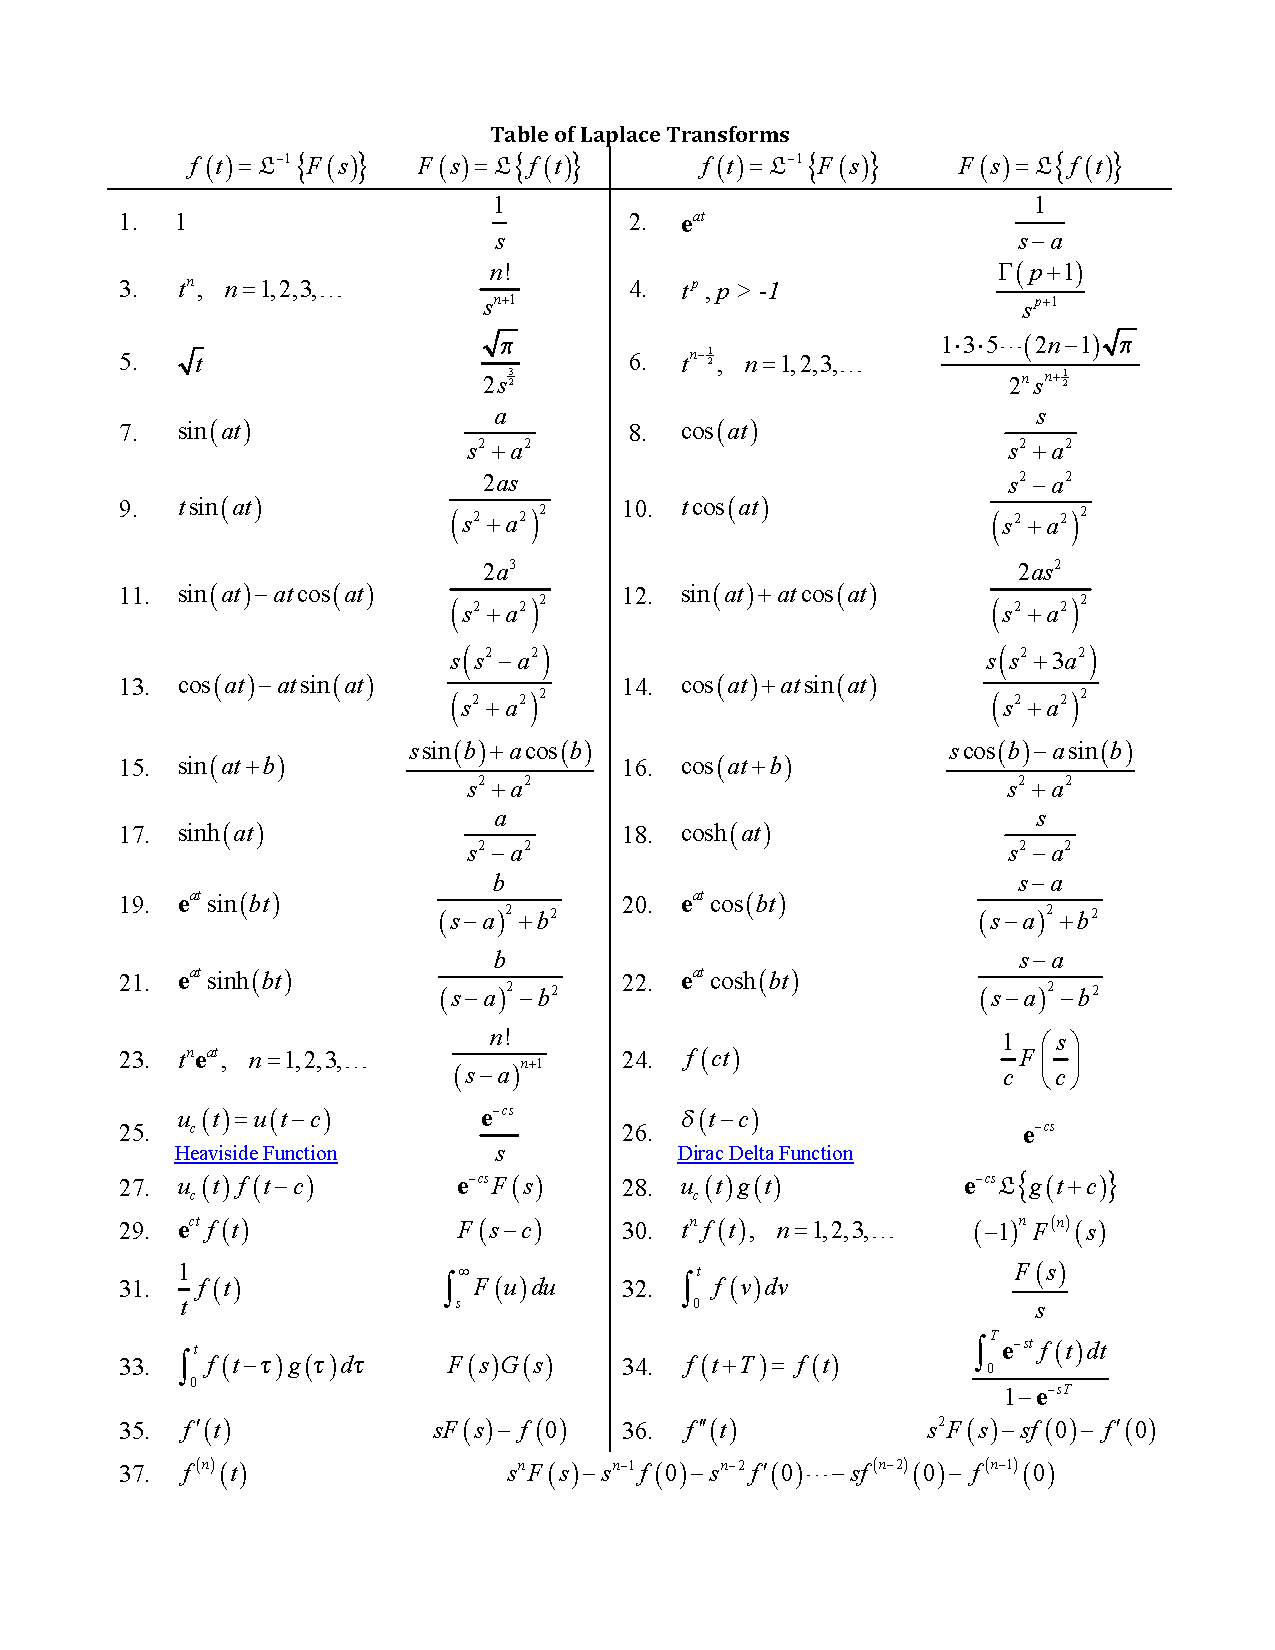
\includegraphics[width=\linewidth]{table.pdf}
\end{center}


\end{document}
